
%***************************************************************************
%
% CreditCruncher - A portfolio credit risk valorator
% Copyright (C) 2004 Gerard Torrent
%
% This program is free software; you can redistribute it and/or
% modify it under the terms of the GNU General Public License
% as published by the Free Software Foundation; either version 2
% of the License.
%
% This program is distributed in the hope that it will be useful,
% but WITHOUT ANY WARRANTY; without even the implied warranty of
% MERCHANTABILITY or FITNESS FOR A PARTICULAR PURPOSE.  See the
% GNU General Public License for more details.
%
% You should have received a copy of the GNU General Public License
% along with this program; if not, write to the Free Software
% Foundation, Inc., 59 Temple Place - Suite 330, Boston, MA 02111-1307, USA.
%
%
% resolution.tex - TeX documentation file
% --------------------------------------------------------------------------
%
% 2005/01/22 - Gerard Torrent [gerard@fobos.generacio.com]
%   . initial release
%
%***************************************************************************

\chapter{Resoluci\'on del problema}
\label{sec:resolution}

TODO: que es lo que esperamos: flexibilidad, resultados finos, paralelismo 
con la valoracion del riesgo de mercado (pe. valoracion de opciones)

%---------------------------------------------------------------------------

\section{Hip\'otesis}

\paragraph{La \'unica fuente de riesgo es el riesgo de impago.}
No se contemplan los riesgos de variaci\'on de tipos de inter\'es, etc.

\paragraph{El tiempo est\'a repartido uniformemente.}
blablabla.

\paragraph{Un fallido no se recupera.}
blablabla.

\paragraph{Las probabilidades de fallido no dependen del tiempo.}
blablabla.

\paragraph{El rating y la recuperaci\'on de un cliente no depende de otro cliente.}
blablabla.


%---------------------------------------------------------------------------

\section{Reparto del tiempo}


%---------------------------------------------------------------------------

\section{El m\'etodo de Monte Carlo}



%---------------------------------------------------------------------------

\section{C\'opulas. Variables aleatorias correlacionadas}

\subsection{Errores comunes sobre la correlaci\'on}

\paragraph{Definici\'on.}
Una copula es la funci\'on de distribuci\'on de un vector aleatorio sobre 
$\Re^n$ donde las funciones de distribuci\'on marginales son $U[0,1]$. 
\begin{displaymath}
C(u_1, \cdots, u_n) = P\{U_1 \leq u_1, \cdots, U_n \leq u_n\}
\end{displaymath}

\paragraph{Proposici\'on.}
$C$ es una c\'opula $\iff C:[0,1]^n \to [0,1]$ y cumple las siguientes 
propiedades:
\begin{itemize}
\item $C(x_1, \cdots, x_n)$ es creciente en cada componente $x_i$
\item $C(1, \cdots, 1, x_i, 1, \cdots, 1) = x_i \quad \forall i \in \{1, \cdots, n\}, x_i \in [0,1]$
\item $\forall (a_1, \cdots, a_n) \in [0,1]^n$ y $\forall (b_1, \cdots, b_n) \in [0,1]^n$ con
$a_i \leq b_i$ se cumple:
\begin{displaymath}
\sum_{i_1=1}^{2} \cdots \sum_{i_n=1}^{2} (-1)^{i_1+\cdots+x_n} C(x_{1i_1},\cdots,x_{ni_n}) \geq 0
\end{displaymath}
\noindent siendo $x_{j1}=a_j$ y $x_{j2}=b_j$ $\quad \forall j \in \{1, \cdots, n\}$
\end{itemize}

\paragraph{Generaci\'on de c\'opulas normales o arquimedianas.}

Sea $(Z_1,\cdots, Z_n)$ un vector aleatorio con marginales $Z_i \sim N(0,1)$ con
\begin{displaymath}
\Sigma = \left( 
\begin{array}{cccc}
1          & \rho_{12} & \ldots & \rho_{1n} \cr
\rho_{21} & 1          & \ldots & \rho_{2n} \cr
\vdots    & \vdots    & \ddots & \vdots   \cr
\rho_{n1} & \rho_{n2} & \ldots & 1
\end{array}
\right)
\end{displaymath}

\noindent siendo $\rho_{ij} = \rho_{ji}$ el coeficiente de correlaci\'on entre 
$Z_i$ y $Z_j$.

\noindent Calculamos la raiz de $\Sigma$ usando el algoritmo de Cholesky. 
De esta forma obtenemos la matriz triengular inferior
\begin{displaymath}
B = 
\left(
\begin{array}{cccc}
b_{11}   & 0        & \ldots & 0       \cr
b_{21}   & b_{22}   & \ldots & 0       \cr
\vdots  & \vdots  & \ddots & \vdots \cr
b_{n1}   & b_{n2}   & \ldots & b_{nn}
\end{array}
\right)
\end{displaymath}

\noindent que cumple $B \cdot B' = \Sigma$

\noindent Generamos una simulaci\'on del vector aleatorio $Y=(Y_1, \cdots, Y_n)'$ 
donde $Y_k \sim N(0,1)$ son variables aleatorias independientes.

\noindent Calculamos $Z = B \cdot Y$. El vector aleatorio resultante, $Z$ tiene
marginales $Z_k \sim N(0,1)$ y se encuentran correlacionadas seg\'un la matriz 
$\Sigma$.

\noindent Calculamos $X = (X_1, \cdots, X_n)'$ de la forma:
\begin{displaymath}
x_i = \Phi^{-1}(y_i)
\end{displaymath}

\noindent donde $\Phi(x) = \int_{-\infty}^{x} \frac{1}{\sqrt{2 \pi}} e^{-t^2} dt$

\begin{figure}[!hb]
\begin{center}
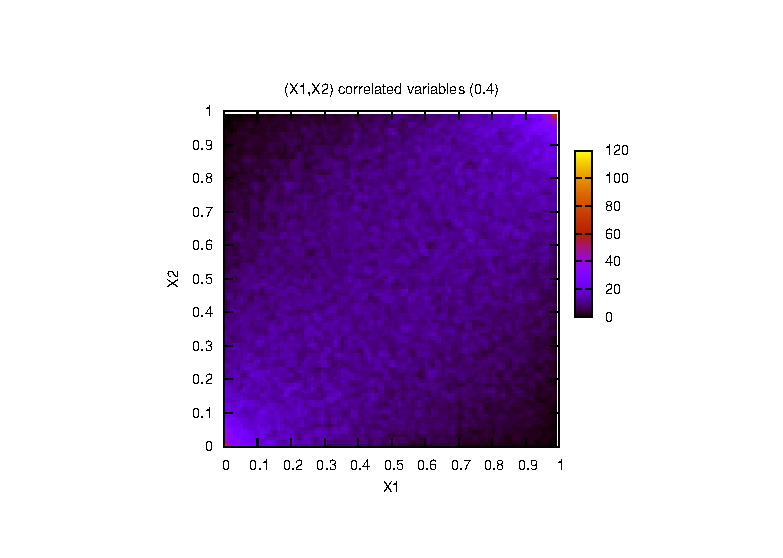
\includegraphics[height=5cm, angle=0]{./images/copula.eps}
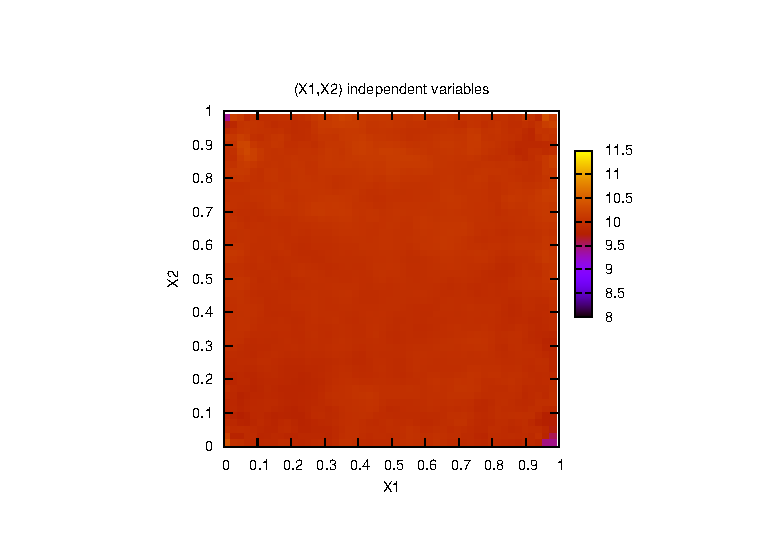
\includegraphics[height=5cm, angle=0]{./images/uniform.eps}
\caption{Bivariate distribution plot with correlation and independent}
\label{copulas}
\end{center}
\end{figure}

%---------------------------------------------------------------------------

\section{Algoritmo de resoluci\'on}

